\documentclass[a4paper]{article}
\usepackage[pdftex]{graphicx}
\usepackage{float}
\usepackage{hyperref}
\usepackage{amssymb}
\floatstyle{ruled}
\newfloat{listing}{hbtH}{lop}
\floatname{listing}{Listing}
\renewcommand{\topfraction}{0.85}   % This sets the percentage for how much floats get from the ‘top’ of the text of a page
\renewcommand{\textfraction}{0}   % This sets a similar percentage for how much of a page needs to be text before no more floats can be placed on that page
\renewcommand{\floatpagefraction}{0.80} % This sets how much of the page must be taken by a float before that page can be ‘all’ floats

\newcommand{\subtypeeq}{\sqsubseteq}
\newcommand{\subtype}{\sqsubset}

\author{Etienne Kneuss\\
\texttt{etienne.kneuss@epfl.ch}
}
\title{Insane: Interprocedural Static Analysis Engine for Scala}
%\bibiographystyle{unsrt}
\begin{document}
\maketitle
\begin{abstract}
  This report presents the work that was done during the winter semester
  2011-2012. It describes the various improvements and refinements that
  were applied to the original analysis.
\end{abstract}
\section{Introduction}
Insane is a pointer and effect analysis for Scala applications. It is meant to
compute and combine modular effects, with various degrees of precision. It was
specifically designed to address higher-order functions -- or equivalently
precise handling of dynamic dispatch. Insane is composed of a combination of
two analyses:

\begin{enumerate}
    \item a precise, intra-procedural but flow-sensitive \textbf{type analysis}
    \item a modular, inter-procedural pointer and \textbf{effect analysis}
\end{enumerate}

\section{Type Analysis}
\subsection{Overview}
Object oriented languages such as Scala implement \emph{dynamic dispatch}: the
target of a method call is only determined at runtime, based on the actual
runtime type of the receiver. This feature is essential in object oriented
languages as it allows subtype polymorphism. Obtaining precise information on
the possible runtime types of those receivers will allow us to construct a
precise call-graph.

Type analysis is responsible to compute an over approximation of the set of
actual concrete types a variable could hold at runtime. Given a variable
\verb=v : T=, we know that its static type \verb=T= already provides a valid
bound on the set of possible concrete types, but this information is not
precise enough in practice. This analysis is designed to improve this static
bound by tracking how allocated objects flow in a procedure and derive more
precise type constraints. We use abstract interpretation using sets of type
constraints as abstract values.

\subsection{Improvements}
The only sensible improvement that was applied to this analysis is the precise
handling of casts. Previously, casting an object would generate a type
constraint corresponding to the type used in the cast. While valid, it is not
precise enough. We re-implemented it using type intersection, as follows:



\subsection{Evaluation}
It is not obvious whether this simple analysis will give interesting results.
The main purpose of this analysis being to compute the call-graph, we will focus
on the improvements obtained for method calls. That is, for each method call,
we compare the number of targets that we obtain with and without refined type
constraints.

The Scala library contains 122'980 method calls at our compiler phase. However,
only 18'611 of them have a non-unique \emph{static} target. We represent
the improvements provided by our analysis using the scatter plot in
Figure~\ref{fig:scatter}. We can clearly see that the improvements are
important. Also, we notice that this analysis is at least as precise as the
static type is: it is only improving the set of targets. In overall we obtain
1'278'384 edges in our refined call graph, instead of 3'554'422 without the
analysis.

\begin{figure}[h]
    \begin{center}
    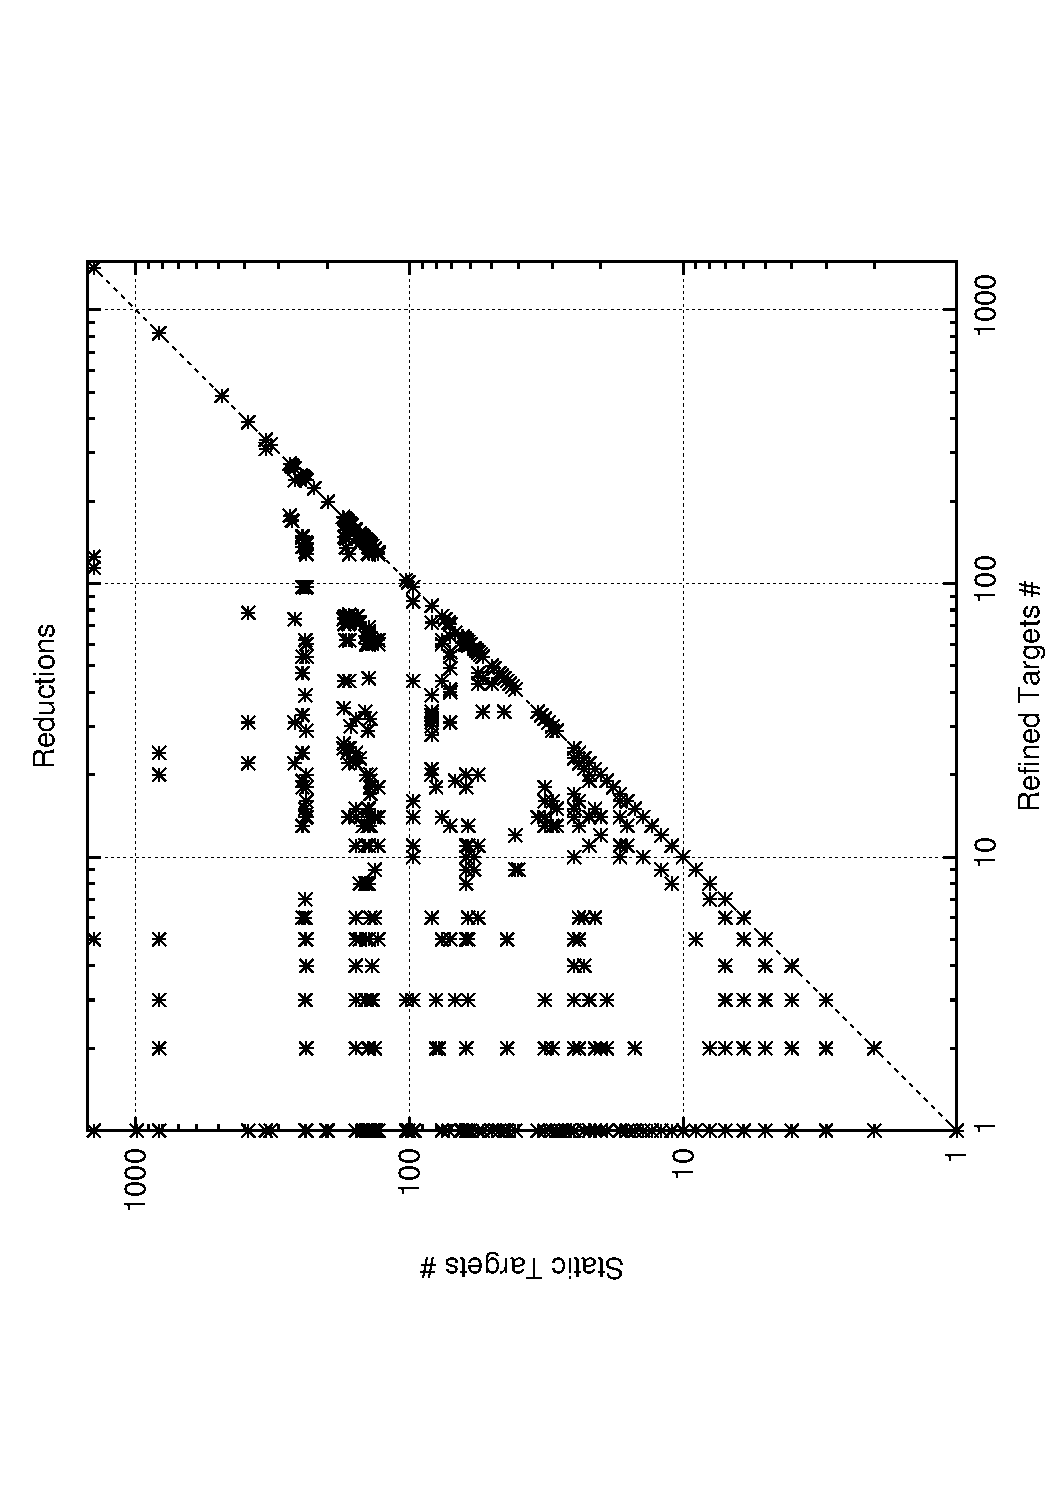
\includegraphics[scale=0.6]{images/scatter}
    \end{center}
    \caption{Improvements due to Type Analysis. Each point represent targets
    computed for one method call. Points on the diagonal represent calls
    without improvements. Points on the Y axis represent calls where the
    analysis reduced the number of targets to a single method.}
    \label{fig:scatter}
\end{figure}

\section{Effect Analysis}


\end{document}
